\section{Appendix A}\label{sec:appendixA}

\subsection{U-Net Appendix}

\begin{figure}[H]
  \begin{center}
    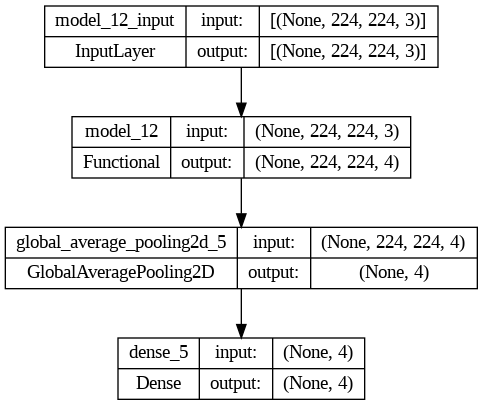
\includegraphics[width=0.35\textwidth]{unet/unetpp_model2.png}
  \end{center}
  \caption{U-Net++ model architecture}\label{fig:unetpp_model}
\end{figure}

Where \texttt{model\_12} is the U-Net++ model with EfficientNetB1 encoder. The Output Layer of \texttt{model\_12} is also used for the segmentation attempt to show what the model deems as the important parts of the image for the classification task.

\subsection{InceptionV3 Appendix}

\begin{figure}[H]
  \begin{center}
    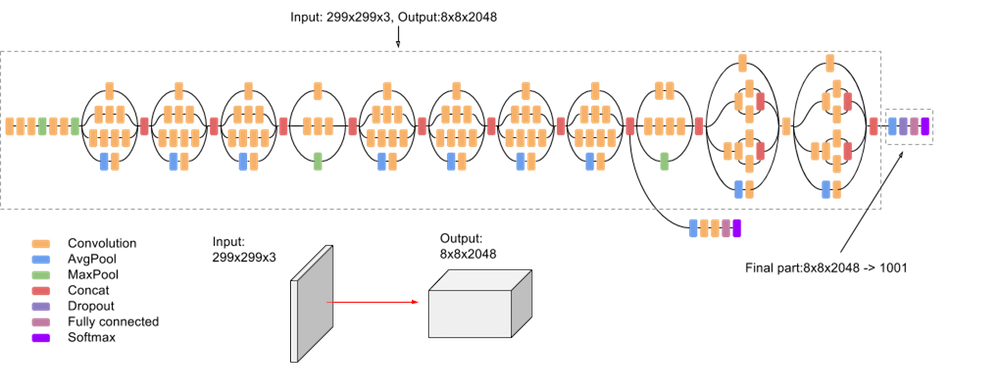
\includegraphics[width=0.6\textwidth]{inceptionv3/inceptionv3_arch.png}
  \end{center}
  \caption{InceptionV3 Architecture}\label{f:inceptionv3_arch}
\end{figure}

This is the architecture of the InceptionV3 model used in the experiments.
